\section{Results}
\label{sec:results}

\subsection{Self-Calibration and Ranking Fidelity}
\label{sec:exp_calibration}

\Cref{tab:calibration} reports rank correlations with RobustBench. On CIFAR-10, our uncalibrated scores achieve $\rho = 0.662$, matching the original paper's reported value of $0.6618$. Self-calibration at $T^* = 2.70$ improves this to $\rho = 0.871$. On ImageNet, where the original paper reported $\rho = 0.800$ without calibration, our uncalibrated scores reach $\rho = 0.900$, and calibration at $T^* = 0.10$ yields $\rho = 1.000$ (perfect ranking). The entire calibration uses only clean accuracies with no adversarial attacks.

\begin{table}[t]
    \caption{Spearman rank correlation ($\rho$) with RobustBench accuracy rankings. Self-calibration matches or exceeds the original attack-based calibration while being fully attack-free.}
    \label{tab:calibration}
    \centering
    \small
    \begin{tabular}{@{}lcccc@{}}
        \toprule
        & \multicolumn{2}{c}{\textbf{CIFAR-10} ($\ell_2$, 17 models)} & \multicolumn{2}{c}{\textbf{ImageNet} ($\ell_\infty$, 5 models)} \\
        \cmidrule(lr){2-3} \cmidrule(lr){4-5}
        & Uncalibrated & Calibrated & Uncalibrated & Calibrated \\
        \midrule
        Original~\citep{li2024greatscoreglobalrobustness} & 0.662 & 0.897\textsuperscript{$\dagger$} & 0.800 & ---\textsuperscript{$\ddagger$} \\
        GF-Score (Ours) & 0.662 & \textbf{0.871} & 0.900 & \textbf{1.000} \\
        \bottomrule
        \multicolumn{5}{@{}l}{\textsuperscript{$\dagger$}\footnotesize Uses C\&W attack for calibration; ours is fully attack-free.} \\
        \multicolumn{5}{@{}l}{\textsuperscript{$\ddagger$}\footnotesize Calibration not performed for ImageNet in the original paper.}
    \end{tabular}
\end{table}

\subsection{Per-Class Robustness Disparity}
\label{sec:exp_disparity}

\textbf{Class vulnerability patterns.} The heatmap in \Cref{fig:heatmap} reveals striking structure. On CIFAR-10, ``cat'' is the most vulnerable class in 13 of 17 models (76\%), while ``automobile'' is the most robust in 10 of 17 (59\%). The remaining worst cases are ``dog'' (4 models) and best cases are ``horse'' (5) and ``truck'' (2). This consistency across diverse training methods suggests that class vulnerability is driven by intrinsic data properties (visual similarity between cats and dogs, distinctiveness of vehicles) rather than training artifacts.

\textbf{Robustness-fairness tension.} \Cref{fig:pareto} plots aggregate GREAT Score against RDI. We observe a clear positive correlation: models with higher aggregate robustness tend to exhibit \emph{greater} class-level disparity. On CIFAR-10, RDI ranges from 0.11 (Wu2020, most fair) to 0.43 (Augustin2020, most disparate), with the most robust models clustered in the high-RDI region. ImageNet shows the same pattern, with RDI between 1.13 and 1.23. Two ImageNet models (Salman\_R18 and Wong2020) have $\mathrm{WCR} = 0.000$, meaning at least one class receives zero certified robustness despite positive aggregate scores. This finding provides new quantitative evidence for the robustness-fairness tension identified qualitatively by \citet{benz2021robustnessoddsfairnessempirical} and \citet{xu2021robustfairfairnessadversarial}.

\begin{figure}[t]
    \centering
    \subfloat[CIFAR-10]{%
        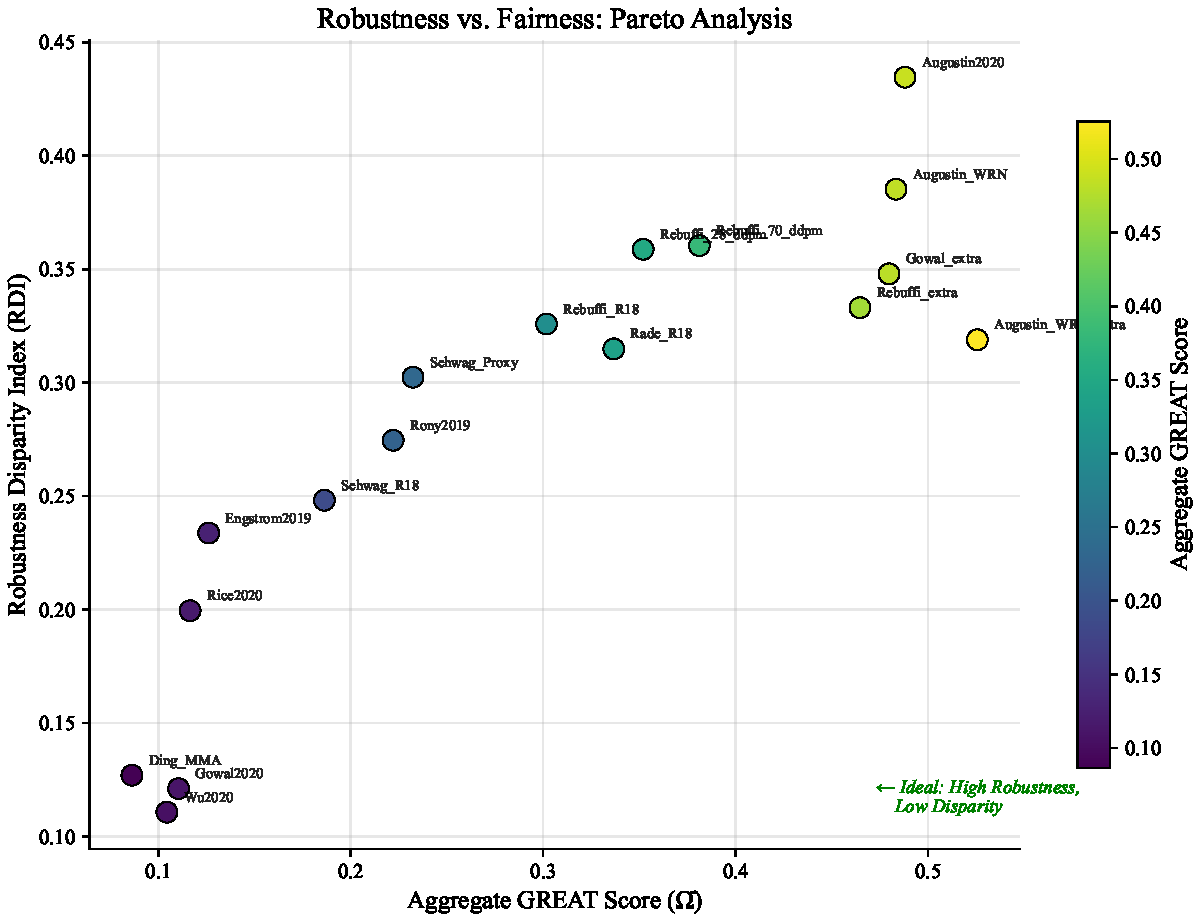
\includegraphics[width=0.48\linewidth]{figures/cifar/pareto.pdf}%
    }\hfill
    \subfloat[ImageNet]{%
        
\includegraphics[width=0.48\linewidth]{figures/imagenet/pareto.pdf}%
    }
    \caption{Aggregate GREAT Score vs.\ RDI. Higher robustness correlates with greater class-level disparity on both datasets, revealing a quantifiable robustness-fairness tension.}
    \label{fig:pareto}
\end{figure}

\textbf{FP-GREAT re-ranking.} When models are ranked by FP-GREAT ($\lambda = 0.5$) instead of the aggregate score, rankings shift substantially. For instance, on CIFAR-10, Augustin2020 drops from 2nd (by aggregate) to 5th (by FP-GREAT) due to the highest disparity ($\mathrm{RDI} = 0.43$), while Wu2020 rises from 16th to 14th due to its low disparity ($\mathrm{RDI} = 0.11$). This demonstrates that fairness-aware ranking provides a meaningfully different and more nuanced view of model quality. Full FP-GREAT rankings and additional figures (disparity bars, vulnerability analysis, calibration curves, RDI concentration plots) are provided in Appendix~\ref{app:figures}.
